\section{Statistics}

\textbf{Basics}
\begin{easylist}[itemize]
\ListProperties(Style*=$\bullet$ , FinalMark={)})
\vspace{-2.0mm}
& Data types = discrete numerical, continuous numerical, and categorical.
\vspace{-3.5mm}
& Cardinality = the number of distinct elements in a set.
\vspace{-3.5mm}
& A statistic summarizes a sample of data, whereas a parameter summarizes the population.
\vspace{-5.0mm}
& Sample mean:
\vspace{-5.0mm}
\begin{equation}
\bar{x} = \frac{1}{n} \sum_{i} x_i
\end{equation}
\vspace{-5.0mm}
& Population mean:
\vspace{-5.0mm}
\begin{equation}
\mu = \frac{1}{n} \sum_{i} x_i
\end{equation}
\vspace{-5.0mm}
& Sample variance:
\vspace{-5.0mm}
\begin{equation}
s^2 = \frac{1}{n-1} \sum_{i} (x_i - \bar{x})^2
\end{equation}
\vspace{-5.0mm}
& Population variance:
\vspace{-5.0mm}
\begin{equation}
\sigma^2 = \frac{1}{n} \sum_{i} (x_i - \bar{x})^2
\end{equation}
\vspace{-5.0mm}
& Median = $50^{\textrm{th}}$ percentile.
\vspace{-3.5mm}
& Visual representations = histograms, time series, and scatter plots.


\end{easylist}

\textbf{Binomial Distribution}
\newline
A random variable has a binomial distribution if:
\begin{easylist}[itemize]
\ListProperties(Style*=$\bullet$ , FinalMark={)})
\vspace{-2.0mm}
& There are a fixed number of trials, $n$.
\vspace{-3.5mm}
& Each trial has two possible outcomes: success or failure.
\vspace{-3.5mm}
& The probability of success, $p$, is the same for each trial.
\vspace{-3.5mm}
& The trials are independent.
\end{easylist}
\vspace{-5.0mm}
\begin{equation}
P(X=k) = {n \choose k} p^{k} (1-p)^{n-k}
\end{equation}
% 
Where
$n$ is the fixed number of trials,
$k$ is the specified number of successes ($0 \leq k \leq n$),\newline
and $p$ is the probability of success on any given trial.
% 
\begin{easylist}[itemize]
\ListProperties(Style*=$\bullet$ , FinalMark={)})
& The mean of $X$ is $\mu = np$.
\vspace{-3.5mm}
& The standard deviation of $X$ is $\sigma = \sqrt{np(1-p)}$.
\vspace{-3.5mm}
& If $np \geq 10$ and $n(1-p) \geq 10$, you can plug $\mu$ and $\sigma$ into a normal distribution.
\vspace{-3.5mm}
& Note that the raw count, $X$, can be converted into a \underline{proportion} by dividing by $n$.
\end{easylist}

\vspace{+3.5mm}
\textbf{Normal Distribution}
\newline
Probability density function:
\vspace{-5.0mm}
\begin{equation}
f(x) = \frac{1}{\sigma \sqrt{2\pi}} \exp{-\frac{1}{2}\Bigg(\frac{x-\mu}{\sigma}\Bigg)^2}
\end{equation}
% 
making the standarizing substitution
\begin{equation}
z = \frac{x-\mu}{\sigma}
\end{equation}
% 
You get a normal distribution with a mean of zero and standard deviation of unity:
\begin{equation}
f(z) = \frac{1}{\sqrt{2\pi}} \exp{-\frac{1}{2} z^2}
\end{equation}
% 
\begin{equation}
\begin{array}{l}
p(-1 < z < +1) = \int_{-1}^{+1} f(z) \, dz \, = 68.27\%
\\ p(-1.96 < z < +1.96) = \int_{-1.96}^{+1.96} f(z) \, dz \, = 95.00\%
\\ p(-2 < z < +2) = \int_{-2}^{+2} f(z) \, dz \, = 95.45\%
\\ p(-3 < z < +3) = \int_{-3}^{+3} f(z) \, dz \, = 99.73\%
\end{array}
\end{equation}

\vspace{+3.5mm}
\textbf{t- Distribution}
\newline
The t-distribution, with $\nu$ degrees of freedom, has the following probability density function:
% 
\begin{equation}
f_{\nu}(t) = \frac{\Gamma(\frac{\nu + 1}{2})}{\sqrt{\nu \pi} \Gamma(\frac{\nu}{2})} \Big(1 + \frac{t^2}{\nu}\Big)^{-\frac{\nu+1}{2}}
\end{equation}
% 
It has a wider distribution than the z-distribution,
however, in the limit $\nu \rightarrow \infty$ it becomes the z-distribution.
The t-distribution is typically used when analyzing the mean of a population.

\vspace{+3.5mm}
\textbf{Central Limit Theorem}
\newline
% Variability in a population is measured in standard deviations.
Sample means vary because you are only sampling a subset of the whole population.\newline
This variability is measured by the \textit{standard error}.
The standard error of the sample mean is
$\sigma_{\bar{x}} = \sigma_{x} / \sqrt{n}$,
where $\sigma_{x}$ is the population standard deviation and $n$ is the sample size.

If you take a sample of a random variable, $x$,
the \textbf{mean} of this sample, $\bar{x}$, is normally distributed:
\vspace{-10mm}
\begin{enumerate}
\item
If $x$ has a normal distribution.
\item
\vspace{-3mm}
If the sample size is large enough $(n > 30)$,
regardless of the distribution of $x$.\newline
$\rightarrow$ This is the Central Limit Theorem.
\end{enumerate}
%
\vspace{-3.5mm}
The z-score is as follows:
\begin{equation}
z = \frac{\bar{x}-\mu_{\bar{x}}}{\sigma_{\bar{x}}} = \frac{\bar{x}-\mu_x}{\sigma_x / \sqrt{n}} 
\end{equation}


\vspace{+3.5mm}
\textbf{Confidence Intervals}
\newline
Statistics (from samples) are used to estimate parameters (belonging to whole populations).
\begin{easylist}[itemize]
\ListProperties(Style*=$\bullet$ , FinalMark={)})
\vspace{-2.0mm}
& Confidence Interval = Statistic $\pm$ Margin-of-error
\vspace{-3.5mm}
& Confidence Level = The probability that this process provides an interval that correctly
$~~~~~~~~~~~~~~~~~~~~~~~~~~~~~~~~~~$ captures the parameter (e.g. for 95\% confidence, $z^{*} = 1.96$).
\vspace{-3.5mm}
& To find the sample size required,
substitute $\mu - x$ for the desired MOE, and solve for $n$.
\end{easylist}

\underline{Population Mean}, when:
\begin{easylist}[itemize]
\ListProperties(Style*=$\bullet$ , FinalMark={)})
\vspace{-2.0mm}
& the population standard deviation, $\sigma$, is known.
\vspace{-3.5mm}
& \textbf{and} $x$ is normally distributed (or $n>30$).
\end{easylist}
% 
\vspace{-5.0mm}
\begin{equation}
\mu_{\textrm{estimate}} = \bar{x} \pm z^{*} \frac{\sigma}{\sqrt{n}}
\end{equation}

\underline{Population Mean}, when:
\begin{easylist}[itemize]
\ListProperties(Style*=$\bullet$ , FinalMark={)})
\vspace{-2.0mm}
& the population standard deviation, $\sigma$, is unknown.
\vspace{-3.5mm}
& \textbf{or} $x$ is not normally distributed, and $n < 30$.
\end{easylist}
% 
\vspace{-5.0mm}
\begin{equation}
\mu_{\textrm{estimate}} = \bar{x} \pm t^{*}_{n-1} \frac{s}{\sqrt{n}}
\end{equation}

\underline{Difference of Two Population Means}, when:
\begin{easylist}[itemize]
\ListProperties(Style*=$\bullet$ , FinalMark={)})
\vspace{-2.0mm}
& the population standard deviations, $\sigma_{1,2,}$, are known.
\vspace{-3.5mm}
& \textbf{and} $x_{1,2}$ are normally distributed (or $n_{1,2}>30$).
\end{easylist}
% 
\vspace{-5.0mm}
\begin{equation}
(\mu_1 - \mu_2)_{\textrm{estimate}} = (\bar{x}_1 - \bar{x}_2) \pm z^{*} \sqrt{\frac{\sigma_1^2}{n_1} + \frac{\sigma_2^2}{n_2}}
\end{equation}

\underline{Difference of Two Population Means}, when:
\begin{easylist}[itemize]
\ListProperties(Style*=$\bullet$ , FinalMark={)})
\vspace{-2.0mm}
& the population standard deviations, $\sigma_{1,2,}$, are unknown.
\vspace{-3.5mm}
& \textbf{or} $x_{1,2}$ are not normally distributed, and $n_{1,2}<30$.
\end{easylist}
% 
\vspace{-5.0mm}
\begin{equation}
(\mu_1 - \mu_2)_{\textrm{estimate}} = (\bar{x}_1 - \bar{x}_2) \pm t_{n_1+n_2-2}^{*} \sqrt{\frac{(n_1-1)s_1^2 + (n_2-1)s_2^2}{n_1+n_2-2}}
\end{equation}

\underline{Population Proportion}, when:
\begin{easylist}[itemize]
\ListProperties(Style*=$\bullet$ , FinalMark={)})
\vspace{-2.0mm}
& $n\hat{p}\geq10$ and $n(1-\hat{p})\geq10$, where $\hat{p}$ is the sample population proportion.
\end{easylist}
% 
\vspace{-5.0mm}
\begin{equation}
p_{\textrm{estimate}} = \hat{p} \pm z^{*} \sqrt{\frac{\hat{p}(1-\hat{p})}{n}}
\end{equation}

\underline{Difference of Two Population Proportions}, when:
\begin{easylist}[itemize]
\ListProperties(Style*=$\bullet$ , FinalMark={)})
\vspace{-2.0mm}
& $n_{1,2}\hat{p}_{1,2}\geq10$ and $n_{1,2}(1-\hat{p}_{1,2})\geq10$.
\end{easylist}
% 
\vspace{-5.0mm}
\begin{equation}
(p_1 - p_2)_{\textrm{estimate}} = (\hat{p}_1 - \hat{p}_2) \pm z^{*} \sqrt{\frac{\hat{p}_1(1-\hat{p}_1)}{n_1}+ \frac{\hat{p}_2(1-\hat{p}_2)}{n_2}}
\end{equation}

\vspace{+3.5mm}
\textbf{Hypothesis Testing}
\newline
A hypothesis test is a statistical procedure that's designed to test a claim (typically about a population parameter).
In general, you assume a claim is true unless you can prove otherwise.
Here is how you do it:
\vspace{-3.5mm}
\begin{enumerate}
\item
\textbf{Set up null and alternative hypotheses.}
\newline
Examples of null hypothesis...~~~~~~~~~~~~$H_0$:~$\mu = 5$,~~$H_0$:~$p_A = p_B$~~(always `equals').
\newline
Examples of alternative hypothesis...~~$H_a$:~$\mu \neq 5$,~~$H_a$:~$\mu < 5$,~~$H_a$:~$p_A \neq p_B$,~~$H_a$:~$p_A > p_B$
\item
\textbf{Collect data via a random sample.}
\item
\textbf{Calculate the test statistic based on the data.}
\newline
We typically use \textit{standard scores} as test statistics.
Here are some examples.

\underline{Population Mean}, when:
\begin{easylist}[itemize]
\ListProperties(Style*=$\bullet$ , FinalMark={)})
\vspace{-2.0mm}
& the population standard deviation, $\sigma$, is known.
\vspace{-3.5mm}
& \textbf{and} $x$ is normally distributed (or $n>30$).
\end{easylist}
% 
\vspace{-5.0mm}
\begin{equation}
z = \frac{\bar{x} - \mu_0}{\sigma / \sqrt{n}}
\end{equation}

\underline{Population Mean}, when:
\begin{easylist}[itemize]
\ListProperties(Style*=$\bullet$ , FinalMark={)})
\vspace{-2.0mm}
& the population standard deviation, $\sigma$, is unknown.
\vspace{-3.5mm}
& \textbf{or} $x$ is not normally distributed, and $n < 30$.
\end{easylist}
% 
\vspace{-5.0mm}
\begin{equation}
t_{n-1} = \frac{\bar{x} - \mu_0}{s / \sqrt{n}}
\end{equation}

\underline{Difference of Two Population Means}, when:
\begin{easylist}[itemize]
\ListProperties(Style*=$\bullet$ , FinalMark={)})
\vspace{-2.0mm}
& the population standard deviations, $\sigma_{1,2,}$, are known.
\vspace{-3.5mm}
& \textbf{and} $x_{1,2}$ are normally distributed (or $n_{1,2}>30$).
\end{easylist}
% 
\vspace{-5.0mm}
\begin{equation}
z = \frac{(\bar{x}_1 - \bar{x}_2) - 0}{\sqrt{\frac{\sigma_1^2}{n_1} + \frac{\sigma_2^2}{n_2}}}
\end{equation}

\underline{Population Proportion}, when:
\begin{easylist}[itemize]
\ListProperties(Style*=$\bullet$ , FinalMark={)})
\vspace{-2.0mm}
& $n\hat{p}\geq10$ and $n(1-\hat{p})\geq10$, where $\hat{p}$ is the sample population proportion.
\end{easylist}
% 
\vspace{-5.0mm}
\begin{equation}
z = \frac{\hat{p}-p_0}{\sqrt{\frac{p_0(1-p_0)}{n}}}
\end{equation}

\underline{Difference of Two Population Proportions}, when:
\begin{easylist}[itemize]
\ListProperties(Style*=$\bullet$ , FinalMark={)})
\vspace{-2.0mm}
& $n_{1,2}\hat{p}_{1,2}\geq10$ and $n_{1,2}(1-\hat{p}_{1,2})\geq10$.
\end{easylist}
% 
\vspace{-5.0mm}
\begin{equation}
z = \frac{(\hat{p}_1-\hat{p}_2)-0}{\sqrt{\hat{p}(1-\hat{p})(\frac{1}{n_1}+\frac{1}{n_2})}}
~~~~~\textrm{where}~~\hat{p} = \frac{c_1 + c_2}{n_1 + n_2}
\end{equation}

\item
\textbf{Find the p-value for your test statistic.}
\newline
A p-value is the probability of getting results at least as strong as yours if $H_0$,
the null hypothesis, were true.

It is determined from the test statistic. It also depends on $H_a$ (the alternative hypothesis):

\begin{figure}[ht]
\centering
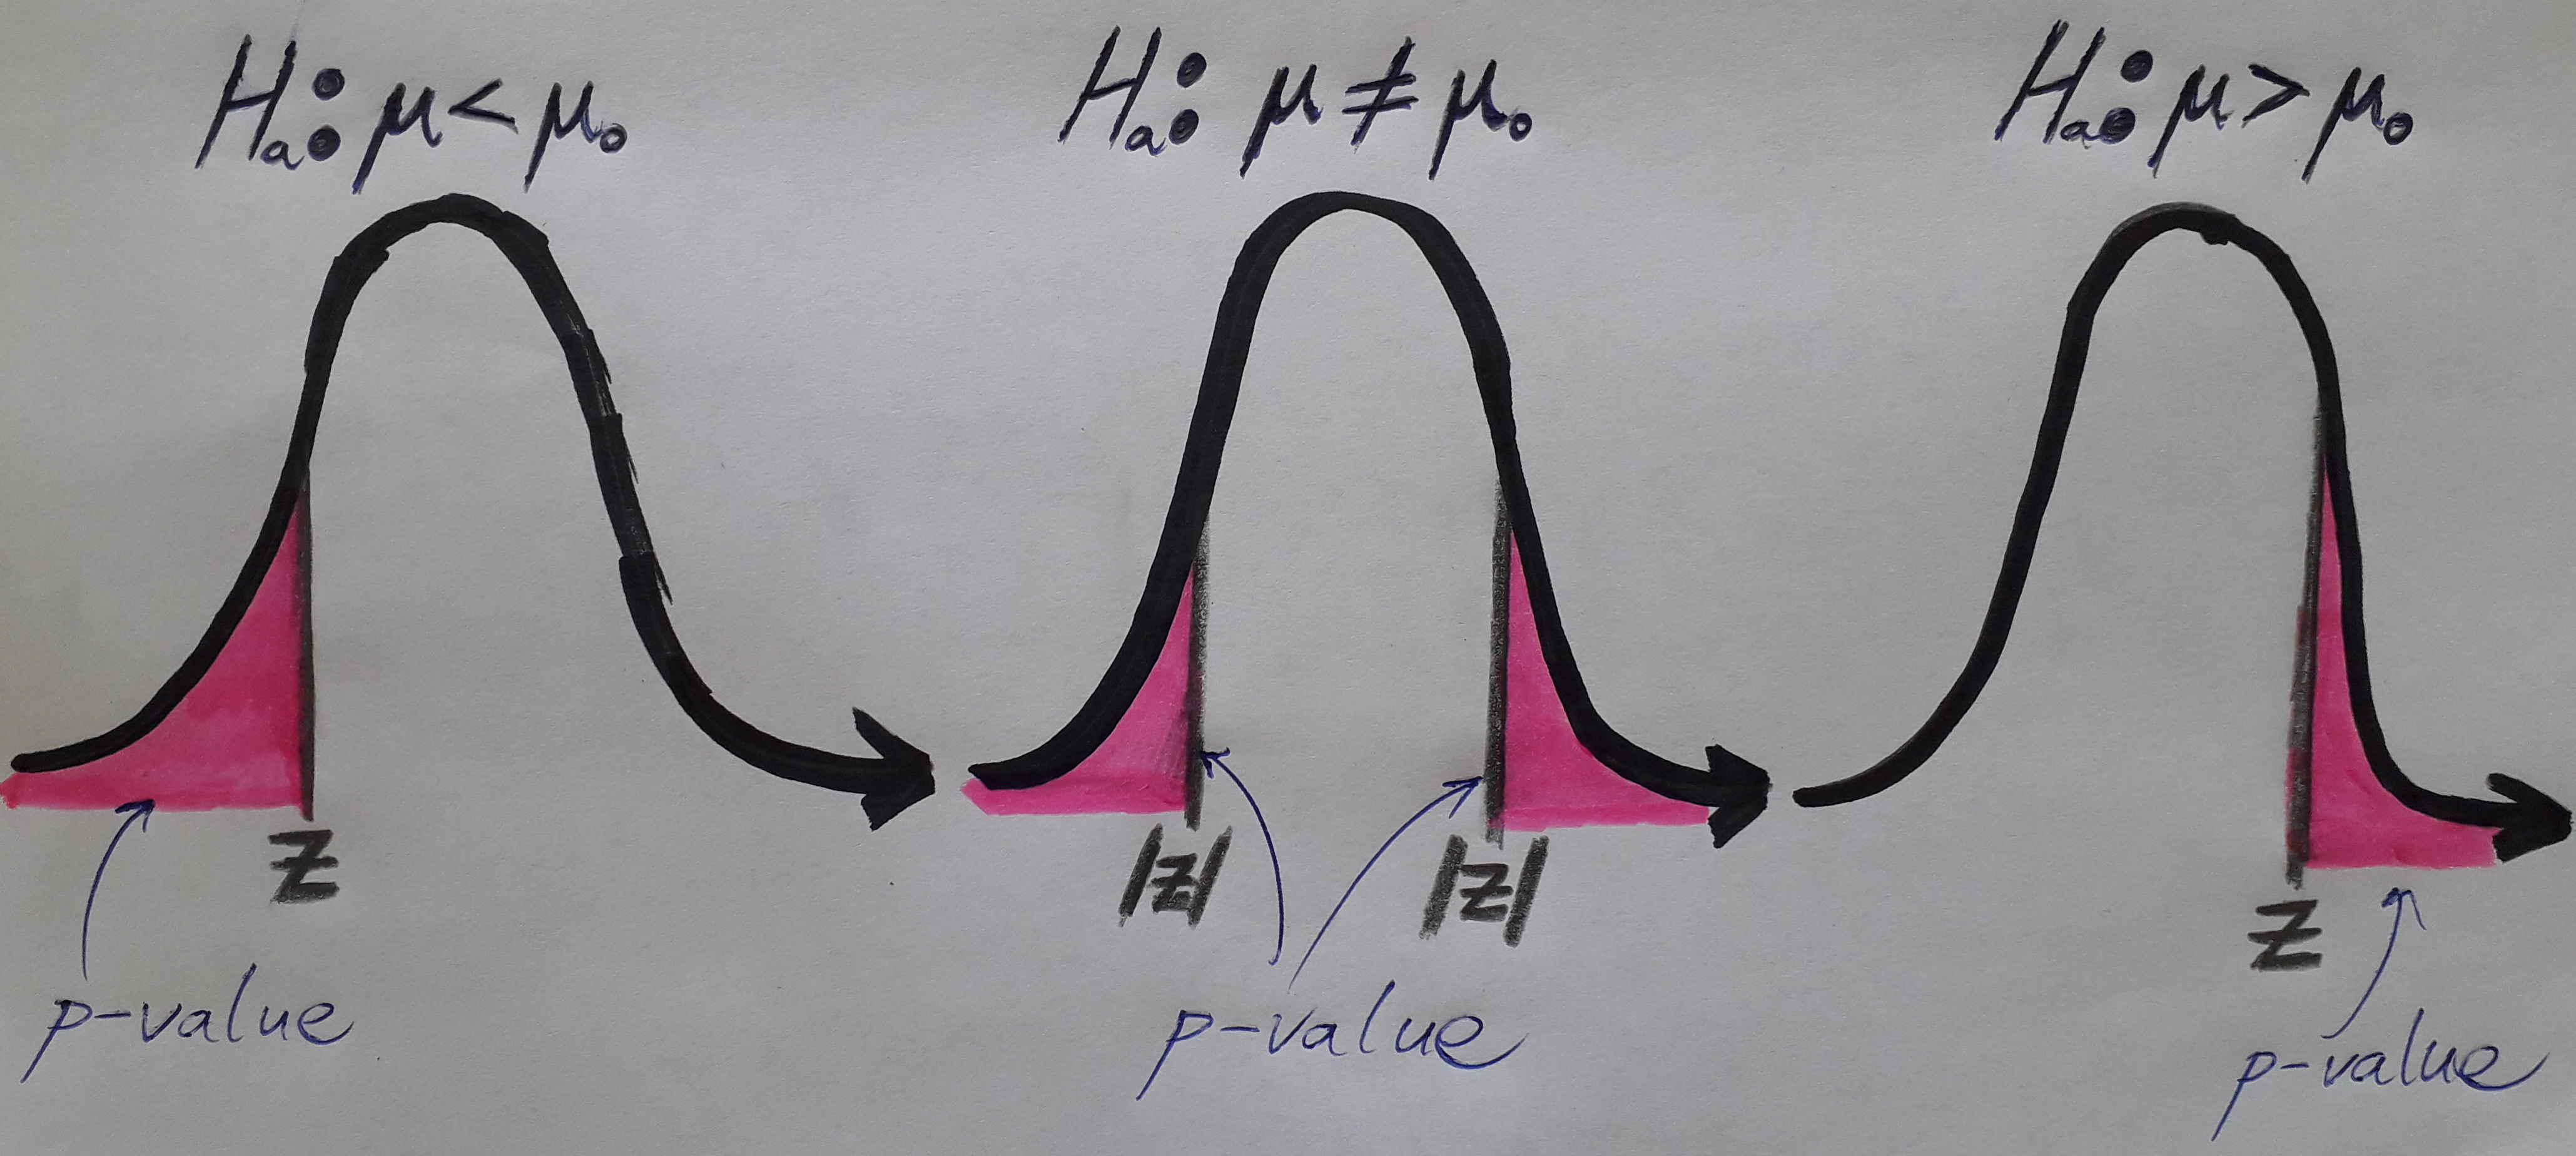
\includegraphics[width=1.00\textwidth]{./images/p_value_edit.jpg}
% \caption{
% % TODO
% }
\label{fig:p_value}
\end{figure}

\item
\textbf{Decide whether or not to reject $H_0$ based on your p-value.}
\newline
If your p-value is less than a \underline{predetermined} significance level ($\alpha$),
then you have enough evidence reject $H_0$. The result is said to be \textit{statistically significant},
i.e. the result is too rare to have occurred by chance if $H_0$ was true.
% 
If your p-value is greater than $\alpha$, you cannot reject $H_0$.
Note that this is different to saying that $H_0$ is true.

A typical significance level is $\alpha = 0.05$.

\end{enumerate}


\newpage